\documentclass[12pt,a4paper,twoside,spanish]{article}      % Libro a 11 pt
\usepackage[utf8]{inputenc}
\usepackage[height=17.5cm,width=13.5cm]{geometry}
\usepackage[Spanish]{babel}         % diccionario
\usepackage{epsfig}         % Graficos Postscript
\usepackage{tabularx}
\usepackage{sectsty}
\usepackage{float}
\usepackage[utf8]{inputenc}
\usepackage{graphicx}
\usepackage{array}
\usepackage{url}




%%%%%%%%%%%%%%%%%%%%%%%%%%%%%%%%%%%%%%%%%%%%%%%
%%%%%%%%%%%%%
%%%%%%%%%%%%% Margenes
%%%%%%%%%%%%%
%%%%%%%%%%%%%%%%%%%%%%%%%%%%%%%%%%%%%%%%%%%%%%%
%%%%% Definimos el maximo tamaño posible.
\marginparwidth 0pt     \marginparsep 0pt
\topmargin   0pt        \textwidth   6.5in
\textheight 23cm

% Margen izq del txt en impares.
\setlength{\oddsidemargin}{.0001\textwidth}

% Margen izq del txt en pares.
\setlength{\evensidemargin}{-.04\textwidth}

% Anchura del texto
\setlength{\textwidth}{.99\textwidth}


%%%%%%%%%%%%%%%%%%%%%%%%%%%%%%%%%%%%%%%%%%%%%%%
%%%%%%%%%%%%%
%%%%%%%%%%%%% Profundidad de enumeracion y tabla de contenidos
%%%%%%%%%%%%%
%%%%%%%%%%%%%%%%%%%%%%%%%%%%%%%%%%%%%%%%%%%%%%%

\setcounter{secnumdepth}{5}
\setcounter{tocdepth}{5}


%%%%%%%%%%%%%%%%%%%%%%%%%%%%%%%%%%%%%%%%%%%%%%%
%%%%%%%%%%%%%
%%%%%%%%%%%%% Nuevos Comandos
%%%%%%%%%%%%%
%%%%%%%%%%%%%%%%%%%%%%%%%%%%%%%%%%%%%%%%%%%%%%%

            %%%%%%%%%%%%%%%%%%%%%%%
            %%%%%%%%%%%%%%%%%%%%%%%
            % Comandos para simplificar
            % la escritura
            %%%%%%%%%%%%%%%%%%%%%%%
            %%%%%%%%%%%%%%%%%%%%%%%

\def\mc{\multicolumn}
            %%%%%%%%%%%%%%%%%%%%%%%
            % Comandos para poder utilizar raggedright en tablas
            %%%%%%%%%%%%%%%%%%%%%%%
\newcommand{\PreserveBackslash}[1]{\let\temp=\\#1\let\\=\temp}
\let\PBS=\PreserveBackslash

% Definir un nuevo tipo de columna con alineación superior
\newcolumntype{L}[1]{>{\raggedright\arraybackslash}p{#1}}




%%%%%%%%%%%%%%%%%%%%%%%%%%%%%%%%%%%%%%%%%%%%%%%
%%%%%%%%%%%%%
%%%%%%%%%%%%% Cuerpo del documento
%%%%%%%%%%%%%
%%%%%%%%%%%%%%%%%%%%%%%%%%%%%%%%%%%%%%%%%%%%%%%


\begin{document}

\def\chaptername{Capítulo}
\def\tablename{Tabla}
\def\listtablename{Índice de Tablas}
\chapterfont{\LARGE\raggedleft}

%%%%%%%%%%%%%%%%%%%%%%%%%%%%%%%%%%%%%%%%%%%%%%%%%%%%%%%%%%%%%%%
%%%%%%%%%%%%%%%%%%%%%%%%%%%%%%%%%%%%%%%%%%%%%%%%%%%%%%%%%%%%%%%
% DISEÑO DE LA PAGINA DEL TITULO
%%%%%%%%%%%%%%%%%%%%%%%%%%%%%%%%%%%%%%%%%%%%%%%%%%%%%%%%%%%%%%%
%%%%%%%%%%%%%%%%%%%%%%%%%%%%%%%%%%%%%%%%%%%%%%%%%%%%%%%%%%%%%%%
\pagestyle{empty}

\begin{titlepage}
\setlength{\parindent}{0cm} \setlength{\parskip}{0cm}

%\raggedleft {\textsf{\textbf{Login del grupo: xxxx}}}

\newcommand{\HRule}{\rule{\linewidth}{1mm}}

\vspace*{2cm}
\HRule \\[0.5cm]
\begin{center}
% Letra lineal y negrita
\textsf{\textbf{\large DESARROLLO DE UN VIDEOJUEGO EN 2 DIMENSIONES\\[0.75cm] SKELLY \& SOULIE \\[0.5cm]}}
\HRule \vspace*{3cm}

\textsf{\textbf{\normalsize Iván García Quintela\\ Ismael Miguez Valero\\ Lola Suárez González\\[5cm]
Grupo 2\\
Contornos Inmersivos, Interactivos y de Entretenimiento\\
Universidade da Coruña \\ 
Curso
2024-2025}}
\end{center}
\end{titlepage}

\cleardoublepage

%%%%%%%%%%%%%%%%%%%%%%%%%%%%%%%%%%%%%%%%%%%%%%%
%%
%% TABLA DE CONTENIDOS
%%
%%%%%%%%%%%%%%%%%%%%%%%%%%%%%%%%%%%%%%%%%%%%%%%

\pagenumbering{Roman}
\tableofcontents
\cleardoublepage


%%%%%%%%%%%%%%%%%%%%%%%%%%%%%%%%%%%%%%%%%%%%%%%%%%%%%%%%%%%%%%%
%%%%%%%%%%%%%%%%%%%%%%%%%%%%%%%%%%%%%%%%%%%%%%%%%%%%%%%%%%%%%%%
%CONTENIDO DEL DOCUMENTO
%%%%%%%%%%%%%%%%%%%%%%%%%%%%%%%%%%%%%%%%%%%%%%%%%%%%%%%%%%%%%%%
%%%%%%%%%%%%%%%%%%%%%%%%%%%%%%%%%%%%%%%%%%%%%%%%%%%%%%%%%%%%%%%

%numeros arábigos
\pagenumbering{arabic} \pagestyle{myheadings} \markboth{Grupo de
prácticas: 02}{Desarrollo de videojuegos}

%indentaciones y espaciado entre párrafos
\setlength{\parindent}{1,5cm} \setlength{\parskip}{0,7cm}

%%%%%%%%%%%%%%%%%%%%%%%%%%%%%%%%%%%%%%%%%%%%%%%%%%%%%%%%%%%%%%%
% ÍNDICE IMPLEMENTADO
%%%%%%%%%%%%%%%%%%%%%%%%%%%%%%%%%%%%%%%%%%%%%%%%%%%%%%%%%%%%%%%


\section{Desarrollo artístico}
\subsection{Antecedentes}
\subsubsection{Ambientación}
Los juegos están ambientados en la época medieval en un mundo de ultratumba donde podrás recorrer el inframundo por el que se han desperdigado las piezas que componen tu ente corpóreo. Posteriormente, te levantarás de entre los muertos para dar caza a aquellos que te arrebataron tu bien más preciado y lo que te mantenía atado a tu mundo: tu propia vida.

\subsubsection{Historia}

La historia del juego sigue a un esqueleto (SKELLY), acompañado de su alma (SOULIE) en la aventura de recuperar sus órganos (plataforma y mazmorras en 2D) y en la búsqueda de venganza (mazmorras 3D). Cada juego tendrá 3 fases.\

En el videojuego 2D “Skelly \& Soulie : Rebuild The Body”, el protagonista comienza con la habilidad de deslizar o empujar objetos, tirar piedras, andar y saltar. En la primera fase recuperará sus pulmones que permitirán saltar más alto. Tras superar la primera fase, recibe sus intestinos como premio, que le darán la posibilidad de colgarse y balancearse de las ramas o atacar a los enemigos. En el segundo nivel recuperará su corazón que le permitirá romper a base de latidos algunos muros, cajas, etc. En el tercer nivel, podrá recuperar su estómago que le sirve para defender o repeler los ataques enemigos. Tras enfrentarse al jefe final, recupera su cerebro y ojos que le permitirán ver y entender el mundo de una nueva forma, lo que nos llevará al desarrollo del segundo juego en 3D.

En el videojuego 3D “Skelly \& Soulie: Revenge Awakened”, Skelly se verá sumido en un viaje de venganza que partirá desde el cementerio, cruzando el bosque y la aldea, hasta el castillo donde se enfrentará a su enemigo con el fin de volver a ser uno con su alma.

\subsection{Personajes}

\renewcommand{\arraystretch}{1.5} % Incrementa la altura de las filas

\begin{table}[H]
\centering
\begin{tabular}{L{2.5cm} L{2cm} L{8cm} L{3cm}}
\hline
\textbf{Nombre} & \textbf{Rol} & \textbf{Descripción} & \textbf{Diseño} \\ \hline
Skelly & Jugador & Es un esqueleto que un día es despertado por su alma y se embarca en la aventura de recuperar sus piezas para poder vengarse y recuperar sus memorias. & \raisebox{-0.7\height}{\includegraphics[width=0.10\textwidth]{images/skelly_memart.jpg}} \\[2mm]
Soulie & Guía & Aparecerá al principio y final de los niveles para proporcionar al protagonista información relevante. & \raisebox{-0.7\height}{\includegraphics[width=0.10\textwidth]{images/soulie_memart.jpg}} \\ \hline
\multicolumn{4}{l}{\textbf{Otras elementos}} \\
\hline
\end{tabular}
\caption{Personajes}
\label{tab:personajes}
\end{table}


\subsection{Otros elementos}

\subsubsection{Enemigos}

\renewcommand{\arraystretch}{1.5} % Incrementa la altura de las filas

\begin{table}[H]
\centering
\begin{tabular}{L{2.5cm} L{2cm} L{8cm} L{3cm}}
\hline
\multicolumn{4}{l}{\textbf{Enemigos 2D}} \\ \hline
\textbf{Nombre} & \textbf{Localización} & \textbf{Descripción} & \textbf{Diseño} \\ \hline
Murciélago  & Común       & Enemigo débil pero molesto que vuela de forma errática. & \raisebox{-0.7\height}{\includegraphics[width=0.10\textwidth]{images/sprite_bat.jpg}} \\[2mm]
Fantasma    & Común       & Enemigo débil que vaga por el mundo. & \raisebox{-0.7\height}{\includegraphics[width=0.10\textwidth]{images/sprite_ghost.jpg}} \\[2mm]
Demonios    & Tercer piso & Estos enemigos pueden atacarte a distancia. & \raisebox{-0.7\height}{\includegraphics[width=0.10\textwidth]{images/sprite_devil.jpg}} \\[2mm]
Jefe Demonio& Final       & Gran demonio que custodia el infierno. & \raisebox{-0.7\height}{\includegraphics[width=0.10\textwidth]{images/demon_memart.jpg}} \\ \hline
\end{tabular}
\caption{Enemigos 2D}
\label{tab:enemigos2D}
\end{table}


\renewcommand{\arraystretch}{1.5} % Incrementa la altura de las filas

\begin{table}[H]
\centering
\begin{tabular}{L{2.5cm} L{2cm} L{8cm} L{3cm}}
\hline
\multicolumn{4}{l}{\textbf{Enemigos 3D}} \\ \hline
\textbf{Nombre} & \textbf{Localización} & \textbf{Descripción} & \textbf{Diseño} \\ \hline
Espantapájaros & Común              & Te lanza hebras de paja que te van drenando la vida. & Diseño a definir \\[2mm]
Hombres lobo   & Común              & Te arañan con sus zarpas y te envenenan. & Diseño a definir \\[2mm]
Aldeanos       & Común              & Te atacan con rastrillos. & Diseño a definir \\[2mm]
Sepulturero    & Jefe Primer Nivel  & Pelea con una pala. & Diseño a definir \\[2mm]
Caballero      & Jefe Segundo Nivel & Pelea con una espada y escudo. & Diseño a definir \\[2mm]
Rey            & Jefe Final         & Usa magia con su cetro. & Diseño a definir \\ \hline
\end{tabular}
\caption{Enemigos 3D}
\label{tab:enemigos3D}
\end{table}


\subsubsection{Objetos destacados}

\renewcommand{\arraystretch}{1.5} % Incrementa la altura de las filas

\begin{table}[H]
\centering
\begin{tabular}{L{3cm} L{3cm} L{3cm} L{3cm}}
\hline
\multicolumn{4}{l}{\textbf{Objetos destacados 2D}} \\ \hline
Icono de vidas & Lápidas & Cofre & Barril \\ 
\raisebox{-0.7\height}{\includegraphics[width=0.10\textwidth]{images/skull_memart.jpg}} & 
\raisebox{-0.7\height}{\includegraphics[width=0.10\textwidth]{images/lapidas_memart.jpg}} & 
\raisebox{-0.7\height}{\includegraphics[width=0.10\textwidth]{images/cofre_memart.jpg}} & 
\raisebox{-0.7\height}{\includegraphics[width=0.10\textwidth]{images/barril_memeart.jpg}} \\[2mm]
Piedras & Ataque Jefe & Intestinos & Corazón\\
\raisebox{-0.7\height}{\includegraphics[width=0.10\textwidth]{images/piedra_memart.jpg}} & 
\raisebox{-0.7\height}{\includegraphics[width=0.10\textwidth]{images/ataquejefe_memart.jpg}} & 
\raisebox{-0.7\height}{\includegraphics[width=0.10\textwidth]{images/instestinos_memart.jpg}} & 
\raisebox{-0.7\height}{\includegraphics[width=0.10\textwidth]{images/corazon_memetar.jpg}} \\[2mm]
Estómago & Pulmones & Cerebro & Llaves de cueva \\ 
\raisebox{-0.7\height}{
\includegraphics[width=0.10\textwidth]{images/estomago.jpg}} & 
\raisebox{-0.7\height}{\includegraphics[width=0.10\textwidth]{images/pulmones.jpg}} & 
\raisebox{-0.7\height}{\includegraphics[width=0.10\textwidth]{images/cerebro_memart.jpg}} & 
\raisebox{-0.7\height}{\includegraphics[width=0.10\textwidth]{images/llaves_memeart.jpg}} \\ \hline
\end{tabular}
\caption{Objetos destacados 2D}
\label{tab:objetos2D}
\end{table}


\renewcommand{\arraystretch}{1.5} % Incrementa la altura de las filas

\begin{table}[H]
\centering
\begin{tabular}{L{3cm} L{3cm} L{3cm} L{3cm}}
\hline
\multicolumn{4}{l}{\textbf{Objetos destacados 3D}} \\ \hline
\multicolumn{3}{L{9cm}}{Al matar enemigos se consigue BoneCoin, que se podrán usar en una tienda (pantalla tipo inventario) en los cambios de nivel.} & 
\raisebox{-0.7\height}{\includegraphics[width=0.10\textwidth]{images/moneda_memart.jpg}} \\[2mm]
\multicolumn{4}{L{12cm}}{Existirán opción de comprar una vida, armadura, remedios.} \\ \hline
\end{tabular}
\caption{Objetos destacados 3D}
\label{tab:objetos3D}
\end{table}



\subsubsection{Lugares}

\renewcommand{\arraystretch}{1.5} % Incrementa la altura de las filas

\begin{table}[H]
\centering
\begin{tabular}{L{3cm} L{6cm} L{5cm}}
\hline
\multicolumn{3}{l}{\textbf{Escenarios 2D}} \\ \hline
\textbf{Nombre} & \textbf{Descripción} & \textbf{Diseño} \\ \hline
Cementerio & Contiene lápidas que se pueden empujar para acceder a plataformas superiores. Fase de desarrollo básicamente horizontal. Tutorial de primeros movimientos, saltos. & \raisebox{-0.7\height}{\includegraphics[width=0.30\textwidth]{images/Cemen2D.jpg}} \\[2mm]
Bosque & Contiene troncos y rocas que se pueden empujar para acceder a las plataformas; hay ramas donde te puedes colgar, subir o balancear. & \raisebox{-0.7\height}{\includegraphics[width=0.30\textwidth]{images/bosqu2d.jpg}} \\[2mm]
Cueva / Infierno & Podrás romper muros para abrirte camino. & \raisebox{-0.7\height}{\includegraphics[width=0.30\textwidth]{images/Cueva2d.jpg}} \\ \hline
\end{tabular}
\caption{Escenarios 2D}
\label{tab:escenarios2D}
\end{table}


\renewcommand{\arraystretch}{1.5} % Incrementa la altura de las filas

\begin{table}[H]
\centering
\begin{tabular}{L{3cm} L{6cm} L{5cm}}
\hline
\multicolumn{3}{l}{\textbf{Escenarios 3D}} \\ \hline
\textbf{Nombre} & \textbf{Descripción} & \textbf{Diseño} \\ \hline
Cementerio & Escenario dominado por el sepulturero. & \raisebox{-0.7\height}{\includegraphics[width=0.30\textwidth]{images/Cementerio.jpg}} \\[2mm]
Bosque & Lugar por el que patrulla el caballero que nos dió muerte. & \raisebox{-0.7\height}{\includegraphics[width=0.30\textwidth]{images/Bosq.jpg}} \\[2mm]
Castillo & Morada del malvado rey que ordenó nuestra muerte. & \raisebox{-0.7\height}{\includegraphics[width=0.30\textwidth]{images/castillo.jpg}} \\ \hline
\end{tabular}
\caption{Escenarios 3D}
\label{tab:escenarios3D}
\end{table}



\subsection{Guion}
Comenzamos con una imagen menú de inicio con tres apartados, nueva partida, cargar partida y opciones.
Opciones nos permite: cambiar dificultad (normal / difícil) Cambiar idioma (Inglés, castellano y gallego) y resolución 
Nueva partida te permite comenzar un juego y partida guardada volver al inicio del nivel donde guardaste, solo se guardan niveles completados.

\subsubsection{Desarrollo 2D}
Introducción, en el cementerio aparece Soulie sobre Skelly.

- Soulie: "Por fin despiertas... pero no estás completo. Alguien te ha despojado de lo que fuiste. Tus entrañas, tu corazón y tu mente están dispersos. Sólo si los recuperas podrás volver a ser tú."

Comienza el nivel, al llegar a la salida del cementerio y recuperar los intestinos.


- Soulie: "Has recuperado algo de ti, pero aún queda un largo camino. La oscuridad se vuelve más densa conforme avanzas."

Y comienza el bosque. Al finalizarlo y recibir el corazón.

- Soulie: "Tu corazón... Aún late con fuerza. Ahora podrás usarlo para destruir ciertos obstáculos que se interpongan en tu camino."

Al entrar en la cueva:

- Soulie: "Cada pieza que recuperas te acerca más a tu esencia, pero también te acerca al infierno... y a quien te arrebató todo."

Al llegar a la mazmorra:

- Diablo: "Te has arrastrado hasta aquí por tu propia voluntad. Qué patético. ¿Crees que un saco de huesos puede desafiarme?"

- Soulie: "Eres más de lo que pareces. Has cruzado la muerte y la desesperación. Recupera lo que es tuyo."

En un cofre oculto en la mazmorra encuentras tu estómago.

- Soulie: Por fín un modo de protegernos de esos molestos ataques. Úsalo para repeler los ataques de los enemigos.

Batalla final contra el demonio. Al vencerlo, el Skelly recupera su cerebro.

- Soulie: "Lo has logrado. Estás completo una vez más... Pero dime, ¿qué harás ahora que recuerdas quién eres?"

El juego termina.


\subsubsection{Desarrollo 3D}
Inicio del juego : 
- Soulie:  ¡Por fin despiertas! Pensé que ibas a quedar enterrado para siempre.
- Skelly:  ¿Dónde estoy?
- Soulie: En el cementerio. Soy yo,  Soulie, tu alma. ¿Estás preparado?, debemos continuar nuestro camino para volver a ser uno.
- Skelly:  ¿Nos separaron? ¿Quién haría algo así?
- Soulie: No lo sé, pero hay que averiguarlo. Para eso, primero tenemos que salir de aquí.


Se desarrolla el nivel hasta llegar a la salida. 
- Sepulturero:  ¡Un muerto caminando! ¡Vuelve a tu tumba o te haré pedazos!

Una vez derrotas a tu enemigo.
- Sepulturero: ¡Cuando llegaste aquí ya estabas muerto, yo solo te enterré! . El caballero Oscuro fue quien te trajo.

Acceso al segundo área 
- Soulie: Algo aquí no me gusta. Hay demasiada calma…
- Skelly: No, nunca debes decir eso.

Al llegar junto al jefe final de esta área.
- Caballero Oscuro: Nadie cruza este bosque sin probar su valía.
- Skelly: ¡Pues veamos quién es más fuerte!

Se desarrolla el combate 

- Caballero Oscuro:  No eres un simple esqueleto... Continúa, guerrero. Pero el destino te espera en la ciudad.

Una vez se derrota al caballero:
- Caballero Oscuro:  Yo solo acataba órdenes de su majestad. Es él, el que ordenó darte caza.

Llegamos a la tercera zona:
- Soulie: No me gusta este lugar... Hay algo oscuro aquí.
- Skelly: Desde aquí puedo ver el castillo, démonos prisa

Nos adentramos en el nivel.
- Rey Espectral: Has llegado lejos... pero tu viaje termina aquí. Fui yo quien separó tu alma de tu cuerpo.
- Skelly: ¿¡Por qué lo hiciste!? ¡Devuélveme mi alma!
- Rey Espectral: Porque un esqueleto con un alma es demasiado poderoso. Pero si crees que puedes vencerme... demuéstramelo.

Se desarrolla la batalla
- Soulie:  ¡Lo logramos! Ahora... ¿qué pasará con nosotros?
- Skelly:  Supongo que... estamos completos otra vez.
- Soulie: Sí. Y ahora, ¿qué sigue?
- Skelly:  Lo que queramos.

Final del juego y créditos.

\clearpage

\section{Desarrollo técnico}

\subsection{Videojuego en 2D}

\subsubsection{Descripción}

En un mundo sumido en la oscuridad, "Skelly \& Soulie" te sumerge en una aventura de plataformas 2D con scroll lateral y vertical, recordando el espíritu de los clásicos de 8 y 16 bits. La historia sigue a Skelly, un esqueleto resucitado de su tumba, y a su inseparable compañero Soulie, el espíritu de su alma. Juntos, emprenden un peligroso viaje a través de bosques sombríos, laberínticas cuevas y hasta los infiernos más profundos, en una misión para recuperar la vitalidad perdida de Skelly.\

Mientras avanzan por escenarios llenos de obstáculos y trampas mortales, Skelly debe recolectar sus órganos dispersos, cada uno dotado de un poder especial que le permite superar barreras y enfrentarse a hordas de monstruos y enemigos temibles. Cada nivel desafiante combina la acción frenética con un toque tétrico y nostálgico, evocando la estética y jugabilidad de aquellos videojuegos clásicos que marcaron una época.\

El juego se distingue por su sistema de scroll dinámico que permite explorar escenarios que se extienden tanto en el plano vertical como el horizontal, donde el jugador debe estar alerta en cada salto y en cada ataque. La atmósfera, impregnada de un aura oscura y siniestra, se complementa con gráficos pixel art elaborados personalmente y una jugabilidad que exige precisión y valentía. "Skelly \& Soulie" es un homenaje a los clásicos de acción de los 80 y los 90.\

\paragraph{Personajes}

\begin{itemize}
    \item Skelly es un esqueleto que, tras años de letargo en su tumba, es despertado por el misterioso impulso de su propia alma. Con un aire melancólico y una determinación oscura, se embarca en una arriesgada aventura para recuperar cada una de sus piezas perdidas. Su apariencia, marcada por restos óseos desgastados y rasgos que insinúan un pasado glorioso y trágico a la vez, refleja la lucha interna entre la venganza y el anhelo de redención. Cada paso que da en su viaje le acerca no solo a la reconstitución de su cuerpo, sino también a la recuperación de memorias olvidadas, que revelarán los secretos de su vida pasada y le permitirán enfrentarse a sus enemigos con una fuerza renovada.\\
    Las partes recuperadas han sufrído algunos cambios con lo establecido inicialmente. Se han eliminado los intestinos ya que estéticamente no se consegía incluírlos en el diseño. Además, para los escenarios finales no era necesario, es más habria dado lugar a que en el segundo nivel no se tuviera que realizar el recorrido inicial. Los pulmones pasan a ser un item recolectable a modo de power up de salto temporal. Al finalizar el primer nivel se consigue el estomago que permite escudarse y al final del segundo el corazón, que permite romper alguna plataforma. Se sigue manteniendo la habilidad de tirar piedras.\\
    La spritesheet contiene los elementos para distintas animaciones:
    \begin{itemize}
        \item Idle: que se refiere a la figura estatica y que cuenta con un solo frame.
        \item Walk: formado por 4 frames que pretende dar sensacion de movimiento.
        \item Shield: dos frames que presentan a Skelly agarrando el estomago y este hinchandose.
       \item Bomb: 4 frames en los que se ve como el corazón crece hasta que lo suelta
        \item Death: o animacion de la muerte del protagonista con 3 frames.
    \end{itemize}
    El sprite original pertenece a \url{https://opengameart.org/content/skeleton} autor Thomaswp y sobre el original se realizaron modificaciones usando Krita (\url{https://krita.org/es/})\\

    \begin{center}
        \raisebox{-0.7\height}{\includegraphics[width=0.8\textwidth]{images_tec2d/skelly_spritesheet.png}}
    \end{center}
    
    \item Soulie es el etéreo guía de Skelly, la manifestación de su alma que aparece al inicio y al final de cada nivel para ofrecer sabiduría y consejos esenciales. Con una presencia casi fantasmal y serena, Soulie actúa como la voz que ilumina el oscuro camino de Skelly, proporcionándole la información necesaria para sortear los peligros y desentrañar los misterios del mundo que le rodea. Soulie es un vínculo vivo entre el pasado y el presente de Skelly, guiándolo hacia la verdad que yace oculta en sus recuerdos.\\
    \begin{center}
        \raisebox{-0.0\height}{
\includegraphics[width=0.2\textwidth]{images_tec2d/Soulie.png}}
    \end{center}
\end{itemize}

\paragraph{Enemigos}

\begin{itemize}

    \item Murciélagos y fantasmas: Estos enemigos de bajo nivel merodean sin rumbo fijo, deambulando por los oscuros cielos y pasillos olvidados. Aunque su presencia puede resultar inquietante, su ataque es mínimo, representando más una molestia que una amenaza real para Skelly.\\
    Sus patrones de movimiento generan las siguientes animaciones:
    \begin{itemize}
        \item Idle: que se refiere a la figura estatica y que cuenta con un solo frame.
        \item Walk: formado por 2 frames que pretende dar sensacion de movimiento.
        \item Death: o animacion de la muerte con 3 frames.
    \end{itemize}
    El sprite original viene de \url{https://opengameart.org/content/ghost-5}, autor StygianChrno, y sobre él se vuelven a realizar modificaciones con el software anteriormente mencionado.

    \begin{center}
        \raisebox{-0.5\height}{\includegraphics[width=0.5\textwidth]{images_tec2d/ghost_sprite_sheet.png}}
    \end{center}
    \begin{itemize}
        \item Idle: que se refiere a la figura estatica y que cuenta con un solo frame.
        \item Walk: formado por 4 frames que pretende dar sensacion de movimiento.
        \item Death: o animacion de la muerte con 3 frames.
    \end{itemize}
    El sprite original proviene de un paquete que proporciona los iconos de ciertos enemigos, \url{https://craftpix.net/freebies/free-chaos-monsters-32x32-icon-pack/?num=1&count=1796&sq=chaos} y los movimientos para la spritesheet se generan de nuevo con Krita.

    \begin{center}
        \raisebox{-0.7\height}{
\includegraphics[width=0.7\textwidth]{images_tec2d/bat_spritesheet.png}}
    \end{center}

    \item Pequeños diablos: A medida que la aventura avanza, surgen estos enemigos que atacan a distancia con proyectiles o ráfagas. Aunque no son invencibles, su capacidad para hostigar al jugador desde lejos añade un nuevo nivel de dificultad y tensión a cada encuentro.\\
    Sus animaciones  son: 
    \begin{itemize}
        \item Idle: que se refiere a la figura estatica y que cuenta con un solo frame.
        \item Walk: formado por 4 frames que pretende dar sensacion de movimiento.
        \item Death: o animacion de la muerte con 2 frames.
    \end{itemize}
    El sprite original proviene también de un paquete que proporciona los iconos de ciertos enemigos, \url{https://craftpix.net/freebies/free-chaos-monsters-32x32-icon-pack} y los movimientos para la spritesheet se generan de nuevo con Krita.

    \begin{center}
        \raisebox{-0.7\height}{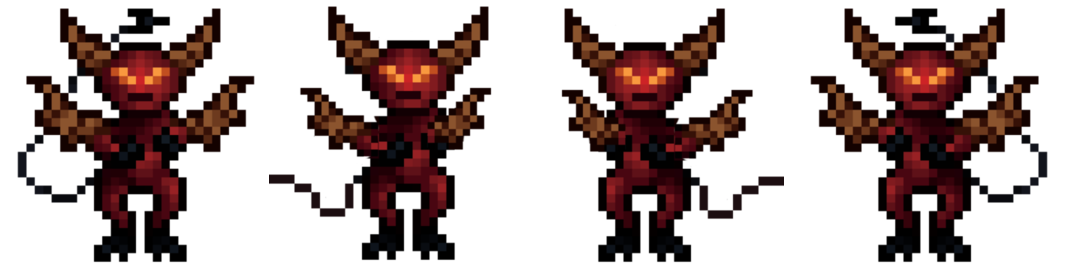
\includegraphics[width=0.6\textwidth]{images_tec2d/devil_spritesheet.png}}
    \end{center}

    \item Demonio Jefe: La culminación de los horrores del inframundo es el Demonio Jefe, un adversario formidable que combina una imponente presencia con ataques devastadores. Este jefe exige paciencia, precisión y reflejos para ser derrotado, ya que representa el pináculo de los desafíos que Skelly debe superar en su oscura travesía.\\
    Sus animaciones son:
    \begin{itemize}
        \item Idle: que se refiere a la figura estatica y que cuenta con un solo frame.
        \item Walk: formado por 2 frames que pretende dar sensación de movimiento.
        \item Melee: 2 frames para crear la sensación de ataque con el tridente
        \item Magic: 4 frames para crear la sensación de la invocación del ataque mágico
        \item Death: o animacion de la muerte con 2 frames.
    \end{itemize}
    El Sprite original pertenece a \url{https://opengameart.org/content/daemon}, pero también fue transformado para adaptarse a nuestras necesidades en el juego.

    \begin{center}
        \raisebox{-0.7\height}{\includegraphics[width=1\textwidth]{images_tec2d/devilking_sprite_sheet.png}}
    \end{center}
\end{itemize}

\paragraph{Objetos}

Los sprites de objetos utilizados finalmente en el desarrollo del videojuego en 2 dimensiones han sido los siguientes:

\renewcommand{\arraystretch}{1.5} % Incrementa la altura de las filas

\begin{table}[H]
\centering
\begin{tabular}{L{3cm} L{3cm} L{3cm} L{3cm}}
\hline
\multicolumn{4}{l}{\textbf{Objetos destacados 2D}} \\ \hline
Icono de vidas & Corazon & Cofre & Piedras \\ 
\raisebox{-0.7\height}{\includegraphics[width=0.10\textwidth]{images/skull_memart.jpg}} & \raisebox{-0.7\height}{\includegraphics[width=0.10\textwidth]{images/corazon_memetar.jpg}} &
\raisebox{-0.7\height}{\includegraphics[width=0.10\textwidth]{images/cofre_memart.jpg}} & \raisebox{-0.7\height}{\includegraphics[width=0.10\textwidth]{images/piedra_memart.jpg}}\\
Estómago & Pulmones & Cerebro & Llave \\ 
\raisebox{-0.7\height}{
\includegraphics[width=0.10\textwidth]{images/estomago.jpg}} & 
\raisebox{-0.7\height}{\includegraphics[width=0.10\textwidth]{images/pulmones.jpg}} & 
\raisebox{-0.7\height}{\includegraphics[width=0.10\textwidth]{images/cerebro_memart.jpg}} & 
\raisebox{-0.7\height}{\includegraphics[width=0.10\textwidth]{images/llaves_memeart.jpg}} \\ \hline
\end{tabular}
\caption{Objetos destacados 2D}
\label{tab:objetos2D}
\end{table}

Para ello se han creado o modificado los siguientes elementos:
\begin{itemize}
    \item Icono de vida.
    \item Icono del botón de pausa.
    \item fondos de los menús.
    \item Animaciones, creadas utilizando la técnica de stopmotion, capturando un cambio por frame; para ello se ha utilizado Blender con la función \texttt{animation2D}, integrando cada elemento y congelando el frame a cada movimiento. (Para lo cual se crearon nuevos frames de movimiento con Krita)
    \item Los fondos de las animaciones: basándose en las capas contenidas en el asset \url{https://opengameart.org/content/parallax-backgrounds} y con Photoshop se han ido construyendo los escenarios. Los objetos que se le añaden, como las plataformas amarillas de guía, o las plataformas del suelo, las trampas de pinchos, árboles, etc., se elaboran en Krita y se van añadiendo al diseño siguiendo la planificación inicial. (añadir si quieres los planos iniciales de nivel)
    \item Plataformas: objeto que escenifica el juego y que se realiza con un rectángulo collider transparente, dado que ya se han integrado en el fondo.
    \item Trampas, pinchos: se sigue la misma dinámica que con las plataformas.
    \item Pulsador y puerta levadiza: objetos creados de forma expresa para el juego usando Krita.
    \item Piedras: \url{https://craftpix.net/freebies/icons-foor-mine-location-32x32-icon-pack}
    \item Bolas de fuego: \url{https://craftpix.net/freebies/icons-for-mine-location-32x32-icon-pack}
    \item Llaves \url{https://opengameart.org/content/golden-and-silver-key-game-item}.
    \item Vidas \url{https://opengameart.org/content/skull-gd}.
    \item Pulmones creados de forma expresa (preguntar a Ivan con qué los hizo).
    \item Corazón creados de forma expresa (preguntar a Ivan con qué los hizo).
    \item Estómago creados de forma expresa (preguntar a Ivan con qué los hizo).
    \item Cerebro creados de forma expresa (preguntar a Ivan con qué los hizo).
    \item Cofre: \url{https://craftpix.net/freebies/free-swamp-objects-pixel-art}
\end{itemize}





\paragraph{Diseño}
% Contenido de diseño en 2D.
Texto de diseño (2D)...

\subsubsection{Escenas}
\paragraph{Escena 1: }
\paragraph{Descripción}
% Detalles de la descripción de la Escena 1.
Texto de descripción de Escena 1...

\paragraph{Modelo}
% Detalles del modelo de la Escena 1.
Texto de modelo de Escena 1...

\paragraph{Detalles de implementación}
% Detalles de implementación de la Escena 1.
Texto de detalles de implementación...

\subsubsubsection{Escena 2: <nombre de la escena 2>}
% Contenido para Escena 2.


\subsubsubsection{Escena 3: <nombre de la escena 3>}
% Contenido para Escena 3.


\subsubsection{Aspectos destacables}
% Contenido de aspectos destacables en 2D.
Texto de aspectos destacables (2D)...

\subsubsection{Manual de usuario}
% Contenido del manual de usuario para el videojuego en 2D.
Texto del manual de usuario (2D)...

\subsubsection{Reporte de bugs}

\paragraph*{Bug de nivel de gravedad bajo:}

\begin{itemize}
    \item \textbf{Las animaciones de la muerte de un enemigo no se renderizan:} cuando un enemigo muere (salvo el enemigo final), las animaciones deberían mostrar cómo los enemigos encogen y desaparecen, pero tan solo se ve la desaparición de los mismos.\\[1mm]
    \textbf{Para replicarlo:} En cualquier nivel del juego, elimina a un enemigo y observa; verás cómo desaparece de la pantalla, pero no se aprecia que su tamaño disminuya ni que el sprite muestre cambios que indiquen muerte.\\[1mm]
    \textbf{Posible solución:} Será necesario revisar que los frames son correctos y que el código que efectúa la muerte del enemigo está pasando por ellos. Se podría dar más tiempo a cada frame o intentar añadir frames a la animación, para ver si se nota algo más.
    
    \item \textbf{Texto extremadamente pequeño en la resolución 720x405 dificulta su lectura:} Para seguir la historia, cada animación contiene una o varias piezas de texto, pero el display de los mismos en la resolución 720x405 es demasiado pequeño para leerse.\\[1mm]
    \textbf{Para replicarlo:} Inicia cualquier nivel en resolución 720x405 y observa la animación.\\[1mm]
    \textbf{Posible solución:} Cambiar el tamaño de la letra o la resolución, o ambas.
\end{itemize}

\bigskip

\paragraph*{Bugs nivel de gravedad medio:}

\begin{itemize}
    \item \textbf{Si coges muy rápido la llave, a veces no se ve que has cogido del cofre:} Si en alguno de los cofres donde se encuentra la llave accedes a él desde la izquierda o desde arriba a la izquierda, la llave entra en tu posesión sin que la veas. Aunque hay efecto sonoro que avisa, estaría bien que se viera que se ha cogido.\\[1mm]
    \textbf{Para replicarlo:} En cualquier nivel (por ejemplo, en el nivel uno, al llegar al árbol con el cofre en las ramas superiores), colisiona con el cofre por la izquierda o por el lado superior izquierdo.\\[1mm]
    \textbf{Posible solución:} Añadir una animación en el personaje que muestre que se ha cogido la llave.
    
    \item \textbf{Los bloques rompibles no son muy obvios:} Apenas se pueden distinguir los bloques rompibles de los normales, salvo que las plataformas estén muy centradas en la pantalla.\\[1mm]
    \textbf{Para replicarlo:} En el nivel tres, revisar los bloques rompibles.\\[1mm]
    \textbf{Posible solución:} Modificar los sprites, añadir efecto sonoro al pisarlos o permitir que la cámara deje más espacio debajo del jugador.
    
    \item \textbf{Reaparición tras la muerte en lugar distinto al debido:} Cuando mueres en la subida del primer nivel, tras haber cogido el cofre de los pulmones, deberías reaparecer donde están los pulmones; pero en ocasiones apareces cayendo en esa zona de la pantalla y puedes acabar chocando contra el fantasma en la caída.\\[1mm]
    \textbf{Para replicarlo:} En el nivel uno, tras coger el cofre con los pulmones, forzar la muerte del personaje.\\[1mm]
    \textbf{Posible solución:} Puede deberse a dónde se sitúa la referencia del rect del personaje.
\end{itemize}

\bigskip

\paragraph*{Bug nivel de gravedad alto:}

\begin{itemize}
    \item \textbf{Muerte contra enemigo invisible:} En ocasiones, un enemigo eliminado vuelve a aparecer y, antes de poder ver el sprite, su caja de colisiones aparece activa, lo que puede causar la muerte del personaje.\\[1mm]
    \textbf{Para replicarlo:} Muévete por donde un enemigo ha muerto.\\[1mm]
    \textbf{Posible solución:} Revisar que el renderizado se active primero antes de estar habilitado para colisiones.
    
    \item \textbf{En el nivel dos puedes quedarte atrapado:} Es posible que si avanzas sin la llave hacia la zona final y se acaba el powerup, quedes atrapado sin posibilidad de volver, salvo esperar a que el enemigo reaparezca y te mate para aparecer en el último cofre cogido.\\[1mm]
    \textbf{Para replicarlo:} Avanza en el nivel dos siempre hacia la derecha y, una vez alcanzado el final, espera a que el powerup se acabe.\\[1mm]
    \textbf{Posible solución:} Rediseñar el final del nivel permitiendo el retroceso o colocar un cofre con powerup en esa zona.
    
    \item \textbf{En el nivel tres puedes quedarte atrapado:} Si no coges la llave, aunque el cofre esté situado para que no se pueda omitir, y rompes los bloques cayendo sin la llave, ya no hay forma de subir, ni siquiera un enemigo para que te mate.\\[1mm]
    \textbf{Para replicarlo:} En el nivel tres, avanza hasta el final sin recoger la llave.\\[1mm]
    \textbf{Posibles soluciones:} Añadir un enemigo que te mate para poder volver a subir (no ideal), permitir que, en ese caso, el personaje pueda subir, o bien hacer que se teletransporte al inicio.
    
    \item \textbf{Colisiones con las plataformas impredecibles:} Cuando saltas muy cerca del borde de una plataforma puede ocurrir un cambio de posición impredecible. Puede ser que rebotes o que te deje montado sobre la plataforma.\\[1mm]
    \textbf{Para replicarlo:} Por ejemplo, en el nivel uno, tras pasar la puerta y comenzar la subida, es posible que al saltar desde la plataforma que tiene el cofre, situada a la derecha, acabes en la plataforma del piso superior.\\[1mm]
    \textbf{Posibles soluciones:} Que la colisión solo ejecute una acción.
    
    \item \textbf{Cofres con vida no siempre devuelven vidas:} Los cofres con vida están diseñados para que el jugador recupere todas las vidas perdidas cuando los recoge. Sin embargo, en ocasiones solo parecen recuperar una vida y, en otras, no devuelven vidas en absoluto.\\[1mm]
    \textbf{Para replicarlo:} No es sencillo, pues no ocurre siempre. En el primer piso, en modo fácil (donde existen más cofres con vidas), pierde dos vidas y prueba a coger un cofre con vidas, repitiendo hasta que suceda el efecto.\\[1mm]
    \textbf{Posibles soluciones:} Tratar las vidas como los pulmones, de modo que solo devuelvan una vida cada uno y que esto esté controlado por un booleano que indique si ya se han cogido.
\end{itemize}

\bigskip

\paragraph{Quality of life:}

\begin{itemize}
    \item Niveles de dificultad no muy nivelados: No existe mucha diferencia entre ellos; como propuesta, modificar el número de vidas de los enemigos según la dificultad, minimizar el tiempo de disparo del diablillo, etc.
    \item Posibilidad de modular el volumen desde el menú de pausa: Aunque de momento se ha dejado fuera y puede ser controlado vía hardware, podría incorporarse en el menú de pausa como una opción.
    \item Inclusión de un marcador para puntuar por cada enemigo eliminado y, con ello, un ranking de partidas.
\end{itemize}

\end{document}

\clearpage

\subsection{Videojuego en 3D}

\subsubsection{Descripción}

\subsubsubsection{Personajes}
% Contenido de personajes en 3D.
Texto de personajes (3D)...

\subsubsubsection{Enemigos}
% Contenido de enemigos en 3D.
Texto de enemigos (3D)...

\subsubsubsection{Objetos}
% Contenido de objetos en 3D.
Texto de objetos (3D)...


\subsubsubsection{Diseño}
% Contenido de diseño en 3D.
Texto de diseño (3D)...

\subsubsection{Escenas}
\subsubsubsection{Escena 1: <nombre de la escena 1>}
\paragraph{Descripción}
% Detalles de la descripción de la Escena 1 en 3D.
Texto de descripción de Escena 1 (3D)...

\paragraph{Modelo}
% Detalles del modelo de la Escena 1 en 3D.
Texto de modelo de Escena 1 (3D)...

\paragraph{Detalles de implementación}
% Detalles de implementación de la Escena 1 en 3D.
Texto de detalles de implementación (3D)...

\subsubsubsection{Escena 2: <nombre de la escena 2>}
% Contenido para Escena 2 en 3D.
Texto de Escena 2 (3D)...

\subsubsubsection{Escena 3: <nombre de la escena 3>}
% Contenido para Escena 3 en 3D.
Texto de Escena 3 (3D)...

\subsubsection{Aspectos destacables}
% Contenido de aspectos destacables en 3D.
Texto de aspectos destacables (3D)...

\subsubsection{Manual de usuario}
% Contenido del manual de usuario para el videojuego en 3D.
Texto del manual de usuario (3D)...

\subsubsection{Reporte de bugs}





%%%%%%%%%%%%%%%%%%%%%%%%%%%%%%%%%%%%%%%%%%%%%%%%%%%%%%%%%%%%%%%
% FINAL DEL DOCUMENTO
%%%%%%%%%%%%%%%%%%%%%%%%%%%%%%%%%%%%%%%%%%%%%%%%%%%%%%%%%%%%%%%


